\documentclass{beamer}
\useoutertheme{lsp}

\usepackage{fontspec,lsptitle,fontawesome,xspace,multicol,booktabs,tikz,eurosym,pgfplots,newtxmath}
\usepackage[normalem]{ulem}
\usetikzlibrary{graphs,arrows,arrows.meta}

\date{28. Januar 2020}

\title{Aufgaben im Verlagswesen und der (nicht)kommerzielle Sektor}
\author[LangSci]{Felix Kopecky}

\begin{document}
\lspbeamertitle
\section{Motivation}

\frame{\frametitle{Über uns}
\begin{itemize}
 \item aktiv seit 2014
 \begin{itemize}
   \item 2014--2016 FU Berlin 
   \item 2016--2018 HU Berlin
   \item 2019--gemeinnützige UG
 \end{itemize}

 \item Monographien und Sammelbände in der Linguistik
 \item alle Bücher Diamond Open Access (CC-BY 4.0) (keine BPC)
 \item Stand heute 114 Bücher veröffentlicht
 \item Ziel: 30 Bücher/Jahr
 \item 25 Reihen; 1017 Supporter; 350 Community Proofreader
 \item Neben Linguisten und Programmierinnen auch eine Betriebswirtin in der Anfangsphase
 \item seit 2019 finanziert durch Konsortial-Modell von Bibliotheken und wissenschaftlichen Gesellschaften (Danke!)
\end{itemize}
}

\frame{\frametitle{\textit{Wer} steckt dahinter?}
\centering\begin{tikzpicture}
\node at (0:0mm) {
\includegraphics[scale=.75]{langsci_logo_nocolor.pdf}};
\node at (0:3cm) {Authors};
\node at (45:3cm) {Proofreaders};
\node at (90:3cm) {Typesetters};
\node at (135:3cm) {Coordinators};
\node at (180:3cm) {Reviewers};
\node at (240:3cm) {Series editors};
\node at (300:3cm) {Press directors};
\end{tikzpicture}
}

\frame{\frametitle{Motivation: Preise}
\begin{block}{Gedankenexperiment (von Martin Haspelmath)}\vspace{\baselineskip}
\centering\begin{tabular}{@{}l@{\hspace{4\tabcolsep}}lllll@{}}
$t_1$& \faBicycle & → & \faWrench & = & €\\
$t_2$& \faBicycle & → & \faWrench & = & €€\\
\multicolumn{6}{c}{$\vdots$}\\
$t_n$& \faBicycle & → & \faWrench & = & €€€€€\\
\end{tabular}
\end{block}\vfill
\begin{block}{Weder \faBicycle\ noch \faWrench\ verändern sich wesentlich.}Ab einem gewissen $t_n$ ist die einzige rationale Reaktion, das \faWrench\ selbst in die Hand zu nehmen!\end{block}
}

\frame{\frametitle{Motivation: Verfügbarkeit}
\begin{block}{Zugriff auf ein OA-Buch kann eingeschränkt sein durch:}
\begin{itemize}
\item schlecht formatierte, nicht zitierfähige HTML-Darstellung
\item nur einzelne Kapitel werden als PDF bereitgestellt, nicht das gesamte Buch
\item verpflichtende, aber sinnlose, Apps zum Lesen der Bücher
\end{itemize}
\end{block}
\begin{block}{WissenschaftlerInnen wollen die Inhalte in \textbf{normalen} Formaten!}
\begin{itemize}
\item Buch als PDF
\item Bibliographie als \texttt{.bib} o.ä.
\item Rohdaten, ...
\end{itemize}
\end{block}
}

\section{Arbeitsteilung}
\frame{\frametitle{Arbeitsteilung bisher}
\begin{block}{}
\centering
\begin{tabular}{ll}
\bfseries Wiss. Community & \bfseries Ext. Dienstl.\\\midrule
  Konzipieren   &    Korrektorat       \\
  Forschen      &    Satz              \\
  Schreiben     &    Druck             \\
  Formatieren   &    Vertrieb          \\
  Begutachten   &    Archivierung      \\
                &    Rechnungslegung  \\
                &    Steuer            \\
                &    Marketing         \\
\end{tabular}
\end{block}
}

\frame{
\frametitle{Arbeitsteilung neu}
\begin{block}{}
\centering
\begin{tabular}{lll}
\bfseries Wiss. Community & \bfseries Community-based publ. & \bfseries Ext. Dienstl. \\\midrule
  Konzipieren   &    Korrektorat     & Druck       \\
  Forschen      &    Satz            & Vertrieb    \\
  Schreiben     &    (Rechnungslegung) & Archivierung \\
  Formatieren   &    Steuer            \\
  Begutachten   &    Marketing         \\
\end{tabular}
\end{block}
}


% \frame{
% \frametitle{Verteilung der Arbeitsschritte auf den akademischen und den privatwirtschaftlichen Bereich}
% Verben in der letzten Folie = derzeit akademisch
% 
% Nomina in der letzten Folie = derzeit privatwirtschaftlich
% 
% Verben in der letzten Folie = zentrale wissenschaftliche Erkenntnisleistung
% 
% Nomina in der letzten Folie = Hilfstätigkeiten. 
% }

\frame{\frametitle{Arbeitsteilung ist sinnvoll}
\begin{block}{ForscherInnen wollen gar nicht die beste Tinte aussuchen.}\end{block}

\begin{block}{VerlagsmitarbeiterInnen wollen gar nicht ins Labor.}\end{block}

\begin{block}{Die optimale Arbeitsteilung kann von Sub-community zu Sub-community unterschiedlich sein.}\end{block}
}

\section{Die Marke}
\frame{\frametitle{Substituierbarkeit}
\begin{block}{Die Wissenschaft sollte nur dann Arbeitsschritte an Dienstleister auslagern, wenn diese \textbf{substituierbar} sind.}

\begin{itemize}
\item Vertrieb A ist zu langsam? Vertrieb über B!
\item Druckerei A druckt schlecht? Wechsel zu B!
\end{itemize}
\end{block}

\begin{block}{Fast alles ist substituierbar, \textbf{nur die Marke nicht}.}

\begin{itemize}
\item \emph{Nature} ist zu teuer? Publizier bei \emph{Neuruppin University Press}!
\end{itemize}
\end{block}
}


% \frame{\frametitle{Die Marke ist wichtig}
% Wissenschaftliche Publikationsprojekte sind gut beraten, Arbeitsschritte an spezialisierte Unternehmen zu vergeben. 
% 
% Was auf keinen Fall aus der Hand gegeben werden darf, ist die Marke. 
% 
% Das Prestige der Marke wird wesentlich durch die zentrale wissenschaftliche Erkenntnisleistung bestimmt. 
% 
% Die Qualität der Tinte oder die Geschwindigkeit der Auslieferung sind im Vergleich dazu unwichtig. Niemand reicht einen Artikel bei einem Verlag ein, weil dieser so schöne Tinte hat.
% 
% [Bild von Bill Clinton]
% 
% }

\frame{\frametitle{Die Marke ist wichtig}
\begin{block}{Das Prestige einer Marke dient oft als Hinweis für die wissenschaftliche Qualität}
\begin{itemize}
\item Das mit der Veröffentlichung einhergende Prestige wird im akademischen CV in Karrierechancen umgerechnet
\item Eine Veröffentlichung mit hoher Prestige verspricht gute Aussichten für Karriere/Anerkennung
\item Deshalb \textbf<2->{können} Preise für Marken mit sehr hohem Prestige in exorbitante Höhen getrieben werden
\item<2-> Aber von WissenschaftlerInnen geführte Verlage \textbf<2->{müssen} die Preise \textbf<2->{nicht} in dieser Art erhöhen.
\end{itemize}
\end{block}
}

\frame{\frametitle{Das Prestige nutzen}
\begin{block}{Die Früchte des Prestiges werden derzeit größtenteils nicht von der Wissenschaft geerntet\pause{} -- obwohl sie von ihr erarbeitet werden.}\end{block}
\begin{block}{Neue Marken müssen wissenschaftliches Prestige erhalten.}
\begin{itemize}
\item Zum Beispiel, indem sie von einer großen Gruppe erfolgreicher WissenachftlerInnen gegründet werden
\item und/oder kurz nach Gründung viel-beachete Werke ankündigen und veröffentlichen.
\item Universitäts-Verlage mit Bindung (1) an einen Ort und (2) zu großem Programm haben es hierbei nicht leicht.
\end{itemize}
\end{block}
}

\section{Fazit}
\frame{\frametitle{Zurückgeben}
\begin{block}{\textit{Community-based} heißt für uns auch, der Community etwas zurückzugeben}
\begin{itemize}
\item Der \LaTeX-Quellcode unserer Bücher ist öffentlich und kann von anderen als Vorlage benutzt werden.
\item Wir verbessern kontinuierlich die Schriftart \textit{Libertinus}, zB ergänzen wir fehlende Glyphen oder verbessern das Kerning.
\item Entwicklung neuer Software-Pakete, zB für den Textsatz von Merkmalstrukturen (AVMs) in \LaTeX.
\item OpenAire-Projekt \textit{Full disclosure}: Veröffentlichung unseres Business models und Cookbooks.
\end{itemize}
\end{block}
}

% \frame{
% \frametitle{It's the brand economy, stupid}
% Verlage verkaufen Prestige, das als symbolisches Kapital auf CVs in Lebenseinkommen umgewandelt werden kann 
% 
% Je höher der Zuwachs an versprochenem Lebenseinkommen, desto höher der Preis, den der Verlag aufrufen kann
% 
% Das Prestige rührt zu einem großen Teil aus der zentralen wissenschaftlichen Erkenntnisleistung
% Nur ein kleiner Teil des Prestiges rührt aus Hilfstätigkeiten
% 
% Aber: die Früchte des Prestiges (\$\$\$) werden derzeit nicht von der Wissenschaft geerntet, sondern von den Hilfstätigkeiten-Dienstleistern (aka Verlage). 
% 
% Diese sabotieren Verbesserungen im Sinne der Wissenschaft (Lingua/Glossa)
% }

\frame{\frametitle{Fazit}
  \begin{itemize}
    \item Dienstleister sind gut, müssen aber substituierbar sein
    \item Die Marke und ihr Prestige sind zentral
    \item Nicht das Rad neu erfinden; fragen Sie jemanden, der sich damit auskennt
    \item Sinnvoller Fußabdruck/\textit{Lean Startup}
  \end{itemize}
}

\frame{\frametitle{Zurück zu den Preisen}
% \begin{block}{Was preislich mit Community-based-Ansätzen möglich ist:}
% Ein Buch kostet bei Language Science Press im Durchschnitt ca. 3500€. (100--1000+ Seiten).
% \begin{itemize}
% \item Linguistische Veröffentlichungen sind vergleichsweise anspruchsvoll herzustellen.
% \item Sammelbände sind wesentlich aufwändiger und wir haben einige davon.
% \item Bei community-externen Verlagen liegen die OA-BPC eher bei 7000--10000€ und es können Aufpreise schon ab 300 Seiten hinzukommen.
% \item In \textit{Nature} liegen die OA-APC für einen Artikel (1--10 Seiten) bei 4380€.
% \end{itemize}
% \end{block}
\centering
\begin{tikzpicture}
    \begin{axis}[
    ybar,
    ymin=0,
    disabledatascaling,
    ylabel=Tausende €/Publikation,
    xtick={0,1,2},
    enlarge x limits={0.25},
    width=.75\linewidth,
    height=5cm,
    xticklabels={LSP, \textit{Nature}, Verlage},
    nodes near coords,
    axis lines*=left,
    tickwidth=0pt,,
    ]
    \addplot+ [lsDarkBlue,fill=lsMidDarkBlue] coordinates {(0,3.5) (1,4.380) (2,7.000)};
    \addplot+ [lsDarkBlue,fill=lsMidDarkBlue] coordinates {(2,11.000)};
    \end{axis}
\end{tikzpicture}
}

\frame{\frametitle{Zurück zu den Preisen}
\begin{block}{Wie ist es möglich, dass...}
\begin{itemize}
\item wir in allen Hinsichten ein gleichwertiges oder sogar besseres Produkt (Textsatz, Zugriff) als community-externe Verlage liefern
\item und der wissenschaftlichen Community etwas zurückgeben
\item aber trotzdem viel weniger kosten?
\end{itemize}
\end{block}
}

\frame{\frametitle{OpenAire \textit{Full disclosure}}

\begin{block}{Download unter \url{langsci-press.org/opendata}}
\hbox{}\hfill
\includegraphics[width=.35\textwidth]{businessmodel.png}\hfill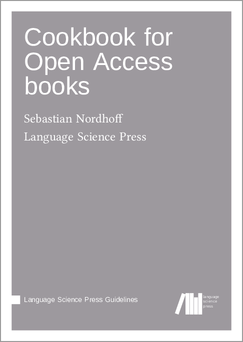
\includegraphics[width=.35\textwidth]{cookbook.png}\hfill\hbox{}
\end{block}
}
\end{document}
